% !TeX spellcheck = en_US
\addscenariosection{1}{Inferno Campaign -- Dungeons and Devils}{2. Steadwick's Fall}{\images/inferno.png}

\begin{multicols*}{2}

\textbf{Author:} Tm335

\textbf{Source:} \href{https://discord.com/channels/740870068178649108/1246353361456861276/1246353361456861276}{Archon Studios Discord}

\textit{Catherine Ironfist has enlisted aid from Bracada and AvLee. 
  She knows we are close to Steadwick. We must occupy Steadwick before she arrives.
  Once we own Erathia's capitol, not even Catherine Ironfist will wrench it from our hands.}

\subsection*{\MakeUppercase{Scenario length}}

This scenario plays out over 16 rounds.

\subsection*{\MakeUppercase{Player setup}}

\textbf{Faction:} Inferno

\textbf{Faction Hero:} Choose any   

\textbf{Starting Resources:}\par
\resources{15}{1}{1}

\textbf{Starting Income:}\par
\resources{10}{2}{0}

\textbf{Starting Units:}

\begin{itemize}
  \item A Few Troglodytes
  \item A Few Evil Eyes
  \item A Pack of Familiars
\end{itemize}

\textbf{Town Buildings:} \svg{bronze} Dwelling, \svg{silver} Dwelling

\vspace*{\fill}\columnbreak

\textbf{Bonus:} Choose one of the following options: 
\begin{itemize}
  \item Add a Pack of Harpies to your hand.
  \item Add a Pack of Magogs to your hand.
  \item Add an Ammo Cart to your hand.
  \item Search (4) the Spell deck.
\end{itemize}

\subsection*{\MakeUppercase{AI hero setup}}

\textbf{Faction:} Castle

\textbf{Enemies:} General Kendal, Charging Heroes

\textbf{General Kendal's Army:} A Pack of Archangels, a Pack of Champions, a Pack of Zealots, a Pack of Crusaders, a Pack of Griffins, a Balista War Machine

\textbf{General Kendal's Deck:} 5 × Might card, 1 × Magic card, 3 × Skill card

\textbf{General Kendal's Spell Deck:} 2 × Haste Spell card

\textbf{General Kendal's Skill:} Artillery Ability card\footnote{For General Kendal, the Artilery Ability card always resolves the Expert effect and the Ballista War Machine activates every time the Artillery Ability card is drawn, as well as at the beginning of a Combat Round.}

\textbf{Charging Heroes' Factions:} Rampart, Tower, Castle

\textbf{Charging Heroes' Armies:} Neutral Army is one level higher than your Hero level (max level VI)\footnote{See page 35, ``Field Difficulty Level Table'' in the Core Rulebook, for further details on the number of Neutral Units you have to draw for this Neutral Army.}.

\textbf{Charging Heroes' Deck:} 2 × Might card, 2 × Magic card

\textbf{Charging Heroes' Spell Deck:} 2 × Slow Spell card\footnote{All the Charging Heroes' Enemies use the same AI and Spell decks. Reset them after each Combat.}.

\subsection*{\MakeUppercase{Map setup}}

Take the following Map tiles and set them up as shown in the scenario map layout:

\textbf{2 × Starting Map tile (I)}
\begin{itemize}
  \item 1 × Inferno (S6)
  \item 1 × Castle (S3)
\end{itemize}

\vspace*{\fill}\columnbreak

\textbf{3 × Far Map tile (II-III)}
\begin{itemize}
  \item 1 × Castle (F3)
  \item 1 × Rampart (F10)
  \item 1 × Dungeon (F2)
  \item 1 × Tower (\#F1)
  \item 1 × Rampart (choose from: F11, F12)
  \item 1 × Necropolis (choose from: F4, \#F6, F7)
\end{itemize}

\textbf{2 × Near Map tile (IV-V)}
\begin{itemize}
  \item 2 × Castle (N3, choose from: \#N3, N6)
  \item 1 × Rampart (N8)
  \item 1 × Necropolis (N4)
\end{itemize}

\subsection*{\MakeUppercase{Heroes placement}}

The Enemy Hero General Kendal is represented by one Castle Faction Hero
model and appears on the center field of the S3 Starting Map tile.

The Castle Charging Hero is represented by one Castle Faction Hero model
and appears on (and owns) the Settlement field of the F3 Map tile.

The Rampart Charging Hero is represented by one Rampart Faction Hero model
and appears on (and owns) the Settlement field of the F10 Map tile.

The Tower Charging Hero is represented by one Tower Faction Hero model
and appears on (and owns) the Settlement field of the \#F1 Map tile.

Place your Main Hero on the center field of the Inferno Starting S6 Map tile.

Place your Secondary Hero, represented by one Dungeon Faction Hero model of your choice,
on the Settlement field of the F2 Map tile. This Settlement produces no resources.

\subsection*{\MakeUppercase{Victory Conditions}}

Defeat all 3 Enemy Controlled Settlements (F3, F10, \#F1), and capture Steadwick (S3) before
Queen Catherine Ironfist arrives at the end of the Round 16.

\subsection*{\MakeUppercase{Defeat Conditions}}

You lose one Combat encounter with your Main Hero (Surrender costs 10 gold, and does not count as a defeat).

You lose your Faction Town on the S6 Map Tile.

You run out of time –- you have time till the end of the Round 16.

\subsection*{\MakeUppercase{Timed Events}}

\textbf{1$^{st}$ Round:}
\begin{itemize}
  \item Read: ``Our underlings have done well. They have managed to raise a volcano
    and erect a fort in a sparsely populated forest just outside of Erathia's border.
    While the Dungeon Overlords make their way underground toward the Erathian capitol,
    you must strike at their allies, the elves of AvLee.'
\end{itemize}

\textbf{2$^{nd}$ Round:}
\begin{itemize}
  \item 
\end{itemize}

\textbf{5$^{th}$ Round:}
\begin{itemize}
  \item 
\end{itemize}

\textbf{10$^{th}$ Round:}
\begin{itemize}
  \item 
\end{itemize}

\textbf{11$^{th}$ Round:}
\begin{itemize}
  \item 
\end{itemize}

\textbf{13$^{th}$ Round:}
\begin{itemize}
  \item 
\end{itemize}

\textbf{15$^{th}$ Round:}
\begin{itemize}
  \item 
\end{itemize}

\textbf{16$^{th}$ Round:}
\begin{itemize}
  \item 
\end{itemize}

\textbf{When you complete the scenario:}
\begin{itemize}
  \item 
\end{itemize}

\subsection*{\MakeUppercase{Additional rules}}

During this ``Inferno'' campaign scenario, the following rules apply:

\begin{itemize}
    \item 
\end{itemize}

\end{multicols*}

% \begin{figure*}[!hb]
%   \newcommand{\maplabel}[1]{}
%   \centering
%   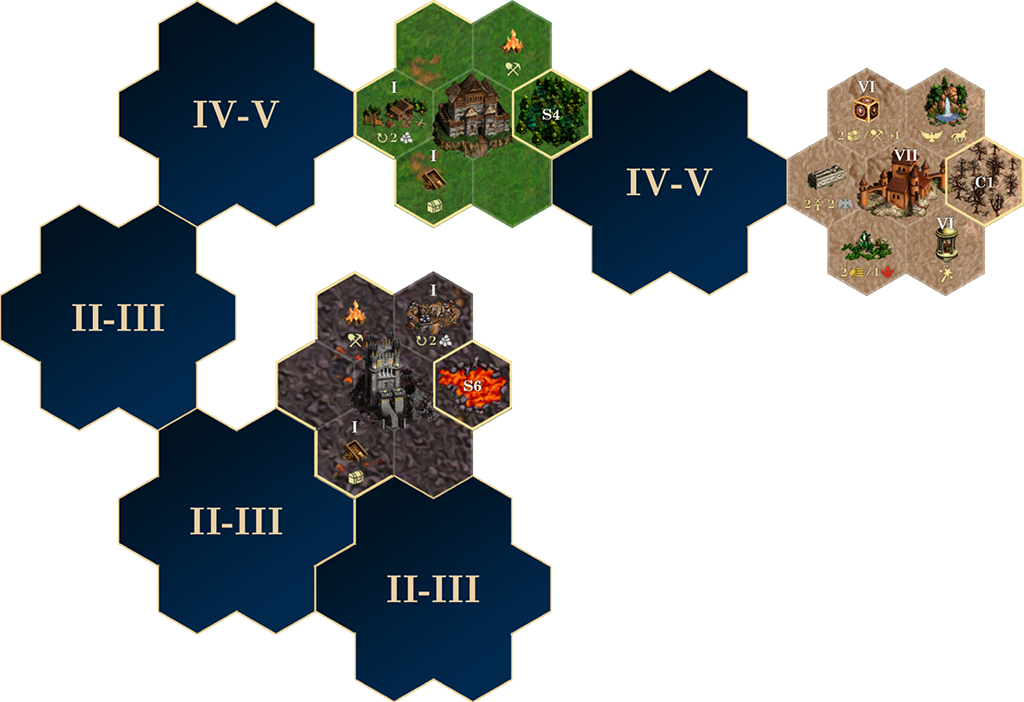
\includegraphics[width=0.8\textwidth]{\_assets/maps/inferno_devilish_plan.png}
%   \begin{tikzpicture}[overlay]
%     \node at (-13, 9.2) {\large{{\textbf{\textcolor{darkcandyapplered}{N8}}}}};
%     \node at (-4, 9.3) {\large{{\textbf{\textcolor{darkcandyapplered}{N7}}}}};
%     \node at (-11.3, 0.2) {\large{{\textbf{\textcolor{darkcandyapplered}{Inferno Map}}}}};
%     \node at (-11.3, -0.5) {\large{{\textbf{\textcolor{darkcandyapplered}{Tiles}}}}};
%   \end{tikzpicture}
% \end{figure*}
